% ****** Start of file apssamp.tex ******
%
%   This file is part of the APS files in the REVTeX 4.1 distribution.
%   Version 4.1r of REVTeX, August 2010
%
%   Copyright (c) 2009, 2010 The American Physical Society.
%
%   See the REVTeX 4 README file for restrictions and more information.
%
% TeX'ing this file requires that you have AMS-LaTeX 2.0 installed
% as well as the rest of the prerequisites for REVTeX 4.1
%
% See the REVTeX 4 README file
% It also requires running BibTeX. The commands are as follows:
%
%  1)  latex apssamp.tex
%  2)  bibtex apssamp
%  3)  latex apssamp.tex
%  4)  latex apssamp.tex
%
\documentclass[%
 reprint,
%superscriptaddress,
%groupedaddress,
%unsortedaddress,
%runinaddress,
%frontmatterverbose, 
%preprint,
%showpacs,preprintnumbers,
%nofootinbib,
%nobibnotes,
%bibnotes,
 amsmath,amssymb,
 aps,
%pra,
%prb,
%rmp,
%prstab,
%prstper,
%floatfix,
10.5pt,
]{revtex4-1}

\usepackage{graphicx}% Include figure files
\usepackage{subfigure}
\usepackage{multirow}
\usepackage{array}
\usepackage{dcolumn}% Align table columns on decimal point
\usepackage{bm}% bold math
%\usepackage{hyperref}% add hypertext capabilities
%\usepackage[mathlines]{lineno}% Enable numbering of text and display math
%\linenumbers\relax % Commence numbering lines

%\usepackage[showframe,%Uncomment any one of the following lines to test 
%%scale=0.7, marginratio={1:1, 2:3}, ignoreall,% default settings
%%text={7in,10in},centering,
%%margin=1.5in,
%%total={6.5in,8.75in}, top=1.2in, left=0.9in, includefoot,
%%height=10in,a5paper,hmargin={3cm,0.8in},
%]{geometry}

\usepackage{xeCJK}
%\setCJKmainfont[ItalicFont={KaiTi}, BoldFont={KaiTi}]{KaiTi}
\usepackage{textcomp}
\usepackage{chemfig}
\usepackage[version=4]{mhchem}
\usepackage{fontspec}
\usepackage{listings}
\usepackage{xcolor}
\usepackage{xcolor} % 定制颜色
\definecolor{mygreen}{rgb}{0,0.6,0}
\definecolor{mygray}{rgb}{0.5,0.5,0.5}
\definecolor{mymauve}{rgb}{0.58,0,0.82}
\lstset{
backgroundcolor=\color{white},      % choose the background color
basicstyle=\footnotesize\ttfamily,  % size of fonts used for the code
columns=fullflexible,
tabsize=4,
breaklines=true,               % automatic line breaking only at whitespace
captionpos=b,                  % sets the caption-position to bottom
commentstyle=\color{mygreen},  % comment style
escapeinside={\%*}{*)},        % if you want to add LaTeX within your code
keywordstyle=\color{blue},     % keyword style
stringstyle=\color{mymauve}\ttfamily,  % string literal style
frame=single,
rulesepcolor=\color{red!20!green!20!blue!20},
% identifierstyle=\color{red},
language=Mathematica,
}

\usepackage[normalem]{ulem}

\newcommand{\chuhao}{\fontsize{42pt}{44.9pt}\selectfont}    % 初号, 1.5倍行距
\newcommand{\xiaochu}{\fontsize{30pt}{40pt}\selectfont}    % 小初, 1.5倍行距
\newcommand{\yihao}{\fontsize{26pt}{36pt}\selectfont}    % 一号, 1.4倍行距
\newcommand{\erhao}{\fontsize{22pt}{28pt}\selectfont}    % 二号, 1.25倍行距
\newcommand{\xiaoer}{\fontsize{18pt}{18pt}\selectfont}    % 小二, 单倍行距
\newcommand{\sanhao}{\fontsize{16pt}{24pt}\selectfont}    % 三号, 1.5倍行距
\newcommand{\xiaosan}{\fontsize{15pt}{22pt}\selectfont}    % 小三, 1.5倍行距
\newcommand{\sihao}{\fontsize{14pt}{21pt}\selectfont}    % 四号, 1.5倍行距
\newcommand{\sihaox}{\fontsize{14pt}{28pt}\selectfont}    % 四号, 1.5倍行距
\newcommand{\banxiaosi}{\fontsize{13pt}{19.5pt}\selectfont}    % 半小四, 1.5倍行距
\newcommand{\xiaosix}{\fontsize{12pt}{24pt}\selectfont} 	% 小四, 1.5倍行距
\newcommand{\xiaosi}{\fontsize{12pt}{18pt}\selectfont}     
\newcommand{\dawuhao}{\fontsize{11pt}{11pt}\selectfont}    % 大五号, 单倍行距
\newcommand{\wuhao}{\fontsize{10.5pt}{10.5pt}\selectfont}    % 五号, 单倍行距
\newcommand{\xiaowu}{\fontsize{9pt}{9pt}\selectfont}    % 五号, 单倍行距

%\usepackage[fntef]{ctexcap}
%\CTEXsetup[number={\chinese{section}、},format={\Large\bfseries}]{section}
%\setCJKfamilyfont{fangsong}{FangSong}                      %仿宋2312 fs  
%\newcommand{\fangsong}{\CJKfamily{fangsong}}  

\usepackage{wrapfig}
\usepackage{fancyhdr}
\usepackage{fancybox}   


\usepackage{tikz}
\usepackage{circuitikz}



\newcommand{\bra}[1]{\langle #1 |}
\newcommand{\ket}[1]{| #1 \rangle}
\newcommand{\bracket}[2]{\langle #1 | #2 \rangle}
\newcommand{\bracketl}[3]{\langle #1 | #2 | #3 \rangle}
\newcommand{\func}{\mathrm \,}
\newcommand{\define}[2]{
	\begin{definition}
	\begin{description}
	\item[#1]
	#2
	\end{description}
	\end{definition}
}

\newcommand{\sch}{Schr\"odinger}
\newcommand{\grad}{\nabla}
\newcommand{\ueq}{\neq}
\newcommand{\celsius}{\ensuremath{^\circ\hspace{-0.09em}\mathrm{C}}}
\newcommand{\unit}[2]{$#1 \, \mathrm{#2}$}

\begin{document}

%\preprint{APS/123-QED}

\title{Measurement of electric potential of silver electrodes}% Force line breaks with \\
%\thanks{A footnote to the article title}% give thanks

\author{Rui Li}
 %\altaffiliation[Also at ]{Physics Department, XYZ University.}%Lines break automatically or can be forced with \\
%\author{Second Author}%
%\email{3160102098@zju.edu.cn}
\affiliation{%
 Qiushi science class (chemistry)\\
 Chu Kochen Honor College
}%

%\collaboration{MUSO Collaboration}%\noaffiliation

%\author{Zong Wei Huang}
% \homepage{http://www.Second.institution.edu/~Charlie.Author}
%\affiliation{
% Second institution and/or address\\
% This line break forced% with \\
%}%
%\affiliation{
%Qiushi science class (chemistry)\\
% Chu Kochen Honor College
%}%
%\author{Delta Author}
%\affiliation{%
% Authors' institution and/or address\\
% This line break forced with \textbackslash\textbackslash
%}%

%\collaboration{CLEO Collaboration}%\noaffiliation

%\date{\today}% It is always \today, today,
             %  but any date may be explicitly specified

\begin{abstract}
Electric potential of several types of silver electrodes is measured using potentiometer, and the density as well as temperature is investigated.
\begin{description}
\item[Keywords]
electric potential, potentiometer
\end{description}
\end{abstract}

%\pacs{Valid PACS appear here}% PACS, the Physics and Astronomy
                             % Classification Scheme.
%\keywords{Suggested keywords}%Use showkeys class option if keyword
                              %display desired
\maketitle

\tableofcontents

\section{Introduction}
Electrode potential is derived from the thermodynamics' second law that for an arbitrary process occurred in a system, the maximum non-volume work is given by
\begin{equation}
W_{\text{non-}pV} \leq  - \Delta G,
\end{equation}
and for a process involving electron transfer, electric work dominates the non-volume work. Faraday pointed out its linearity towards the amount of electrons transferred, as is natural in electric circuits,
\begin{equation}
W_{\text{non-}pV,\text{max}} = - \Delta G = nFE
\end{equation}
where $n$ is the total amounts of electrons transferred, $F$ the Faraday constant representing electric charges of 1 mol electrons, and $E$ represents the electric potential in the circuit provided by the reaction. Thus it is evident that Any reaction that involves electron transfer and a decrease in Gibbs free energy can be applied as an electric power source.

Nernst equation is deduced in the system of chemical equilibrium, from the equation of which was deduced in the former report,
\begin{equation}
 \Delta G_m = \Delta G^\ominus +  RT \ln Q = \Delta G_m^\ominus + RT \ln{\frac{\alpha_\text{product}^{c_i}}{\prod\alpha_\text{reactant}^{c_j}}}
 \end{equation}
 and when decomposing it into half-electrode reactions for oxidants and redox, combining it with the Faraday equation, it is deduced that
 \begin{equation}
 E_\text{red} = E^\ominus_\text{red} -\frac{RT}{zF} \ln{Q'} = E^\ominus_\text{red} - \frac{RT}{zF} \ln{\frac{\alpha_\text{red}}{\alpha_\text{Ox}}}
\end{equation}
where $\alpha$ represents the fugacity of the matter in the solution, and $z$ the amount of electrons per mole of reaction that transferred. The same can be deduced for the redox reaction.

According to Kirchhoff's circuit laws, the current will cause an decrease in the measurement of the potential of a battery using simple electric circuits due to inevitable resistance for the battery. Thus an apparatus that can measure a potential with no current through the battery needs to be adopted, linear sweep vltammetry as one of the examples. The apparatus in this experiment is much simpler, involving several variable resistances with battery that provides a standard electric potential, which can help deduce the electric potential of the target battery according to the Kirchhoff's circuit laws.

\section{Methods and procedures}
A series of standard solution of \ce{KCl} and standard solution of \ce{AgNO3} in different concentrations was prepared respectively. Each battery consists of a pair from four electrodes - saturated calomel electrode in saturated KCl solution, silver chloride electrode in different concentration of \ce{KCl} solution, silver electrode in different concetration of \ce{AgNO3} solution - is measured using Model UJ-25 high voltage DC potentiometer. The electrric potential of battery that consists of saturated calomel electrode in saturated KCl solution and silver chloride electrode in 0.0900 M of KCl solution is measured at different temperatures. 

\section{Result and analysis}

\begin{table}
\centering
\caption{The potential of the cells of different electrodes measured at 25 \celsius using potassium nitrate as the salt bridge}
\begin{tabular}{c|ccccc}\hline
Group & \multicolumn{5}{c}{$c$/M} \\\hline
A &  0.1116 & 0.0832 & 0.06929 & 0.06041 & 0.05454 \\
B &   0.4373 & 0.4627 & 0.4722 & 0.4833 & 0.4917 \\
C &  0.2086 & 0.3835 & 0.4080 & 0.4288 & 0.4339 \\
D &  0.05658 & 0.03192 & 0.01917 & 0.01133 & 0.005567 \\\hline
\end{tabular}

\begin{flushleft}
A:Hg|\ce{Hg2Cl2},KCl(Sat.)||KCl($c$),AgCl|Ag

B:Hg|\ce{Hg2Cl2},KCl(Sat.)||\ce{AgNO3}($c$)|Ag

C:Ag|AgCl,KCl($c$)||\ce{AgNO3}($c$)|Ag

D:Ag|\ce{AgNO3}($c$)||\ce{AgNO3}(0.100 M)|Ag
\end{flushleft}
\label{table}
\end{table}


\begin{table}
\centering
\caption{The potential of Hg|\ce{Hg2Cl2},KCl(Sat.)||KCl(0.09 M),AgCl|Ag measured at different temperatures using potassium nitrate as the salt bridge}
\begin{tabular}{c|ccccc}\hline
T/K & 298.15 & 303.15 & 308.15 & 313.15 & 318.15  \\\hline
E/V & 0.054537 & 0.055457 & 0.055823 & 0.055947 & 0.056093 \\\hline
\end{tabular}
\label{table2}
\end{table}


\begin{figure}
\centering
\subfigure[A]{
	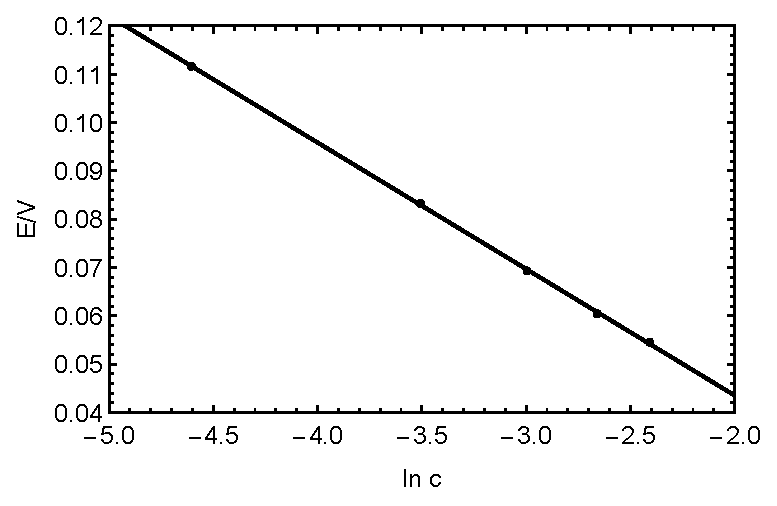
\includegraphics[width=0.22\textwidth]{figures/electropotential1.eps}
}
\subfigure[B]{
	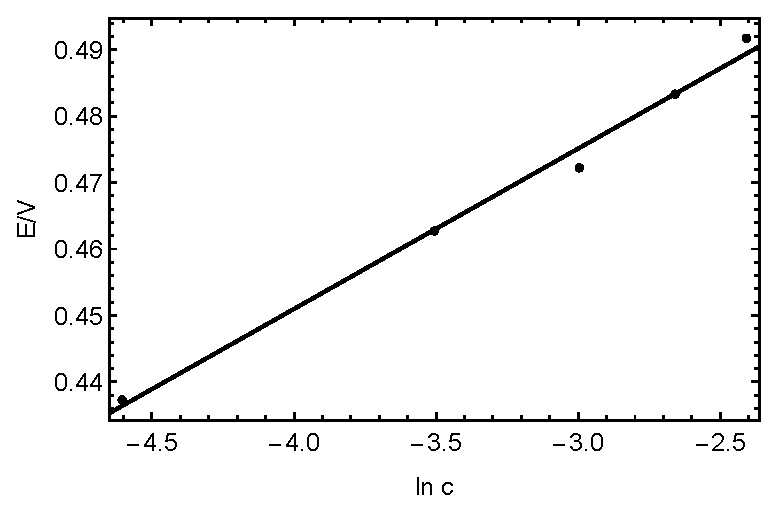
\includegraphics[width=0.22\textwidth]{figures/electropotential2.eps}
}
\subfigure[C]{
	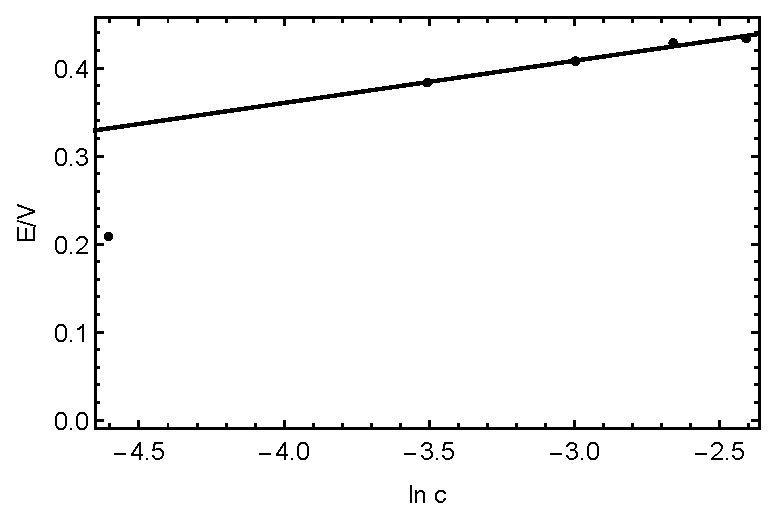
\includegraphics[width=0.22\textwidth]{figures/electropotential3.eps}
}
\subfigure[D]{
	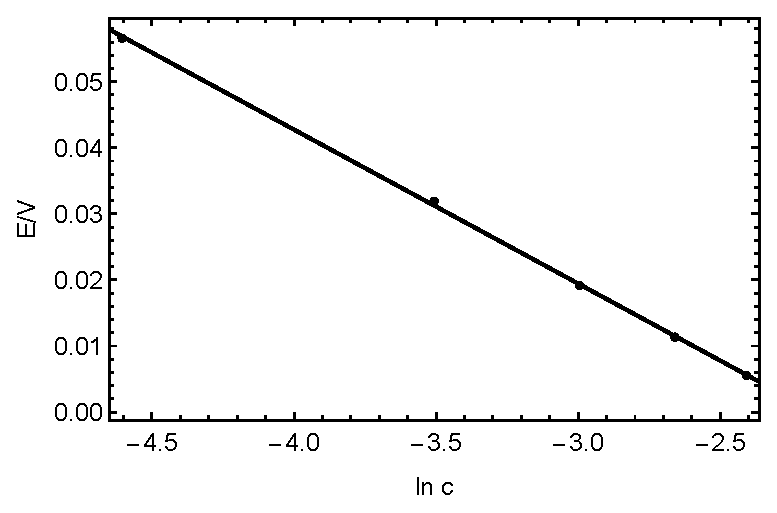
\includegraphics[width=0.22\textwidth]{figures/electropotential4.eps}
}
\caption{The $E$-$\ln{c}$ curve of the cells of different electrodes measured at 25 \celsius~using potassium nitrate as the salt bridge}
\label{figure}
\end{figure}

\begin{figure}
\centering
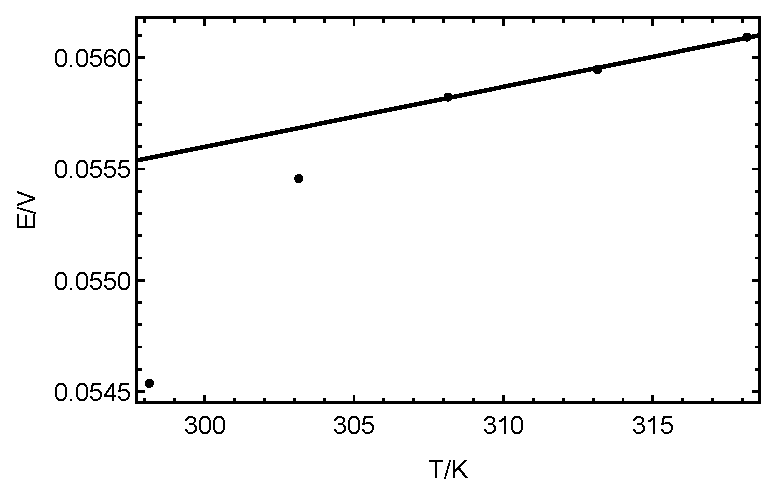
\includegraphics[width=0.4\textwidth]{figures/batterytemp.eps}
\caption{The E-$T$ plot of the potential of saturated calomel electrode combined with silver chloride electrode in 0.09 M KCl measured at different temperatures using potassium nitrate as the salt bridge}
\label{batterytemp}
\end{figure}

The data is shown in Table.\ref{table},\ref{table2}, with figures shown in Fig.\ref{figure},\ref{batterytemp}. Relatively nice linearity is obtained in Fig.\ref{figure}, where the lines are interpreted as
\begin{equation}
\begin{cases}
E_A = -0.00880485 - 0.0261599 \ln{c} \\
E_B = 0.547491 + 0.024127 \ln{c} \\
E_C = 0.552076 + 0.0478942 \ln{c} \\
E_D = -0.0504885 - 0.0233089 \ln{c}
\end{cases}
\end{equation}
with
\begin{equation}
\begin{cases}
R^2_A = 0.999794 \\
R^2_B = 0.991412 \\
R^2_C = 0.984017 \\
R^2_D = 0.999645
\end{cases}
\end{equation}
if excluding the error point in the C group. Substituting $c$ with 1, it is easily obtained that
\begin{equation}
\begin{cases}
E^\ominus_\text{AgCl/Ag} = -0.008805 \, \mathrm{V} \\
E^\ominus_\text{\ce{Ag+}/Ag} = 0.5475 \, \mathrm{V} 
\end{cases}
\end{equation}
in the reference to saturated calomel electrode. Subtracting them gives 0.5563 V, which is identical to the result from the C group (0.5521 V). The slopes deviate slightly from $RT/nF$, namely 0.02569, which might be attributed to limited conductance of the ions in the solution that influences the measurement, and inevitable consumation of the reactant during the measurement. It also gives
\begin{equation}
K^\ominus(\text{AgCl}) = \exp{\frac{-nFE}{RT}} = 2.535 \times 10^{-9}
\end{equation}
which also differs from the standard data($1.8\times 10^{-10}$), which owes itself to the non-one fugacity coefficient of the ions in the solution. 

Data from D group reveals the linearity of the electrode potential towards $\ln{c}$. However, it returns 0.003182 when replacing $c$ to $0.1$ in the formula, which contradicts the general truth that there is no difference of potential between to solution of the same concentration, nevertheless it is not appropriate to ignore. Errors might arise from the factors that have been listed above.

It fails to give linearity in Fig.\ref{batterytemp}, which might be due to non-zero gradient of temperature over the system, especially in the salt bridge, which is outside the thermostat. It affects the fugacity of the ions as well as producing flows of the solution, which is certain to cause unpredictable errors. Picking the last three data points to fit a straight line returns
\begin{equation}
E = 0.0474993 + 0.000027 T
\end{equation}
which is of low confidence. Considering that
\begin{equation}
\Delta_r G_m = \Delta_r H_m - T\Delta_r S_m,
\end{equation}
it can be interpreted that for the cell Hg|\ce{Hg2Cl2},KCl(Sat.)||KCl(0.09 M),AgCl|Ag there is
\begin{equation}
\begin{cases}
\Delta_r G_m = 5360 \,\mathrm{J/mol}\\
\Delta_r S_m = 2.605 \,\mathrm{J/(K\cdot mol)} \\
\Delta_r H_m = 4583 \,\mathrm{J/mol}
\end{cases}
\end{equation}
However, the line is too far from the data point of 25 \celsius, indicating the indifference of calculating $\Delta_r G_m,\Delta_r S_m,\Delta_r H_m$ as well as correcting the density of \ce{Cl-}.







\end{document}

\begin{figure}
\centering
\begin{circuitikz} 
 \draw (0,0) node[spdt,xscale=1,yscale=-1,anchor=in](Swp){SW};
 \draw (Swp.out 1) node[anchor=west] to [battery1]{$E_n$}(-4,0)
 	to [short] (-4,12);
 \draw (Swp.in) 
 	to [nos]{K} (0,5)
 	to [ammeter] (0,10)
 	to [vR]{R_n} (-4,10);
 \draw (4,12) 
 	to [vR]{$R_p$} (0,12)
 	to [battery1]{$E_w$} (-4,12);
 \draw (0,10) 
 	to[american potentiometer,n=pot]{R_x} (4,10)
 	to[short] (4,12);
\draw (pot.wiper) to (4,0);
\draw (4,0) to (Swp out 2) node[anchor=east];
\end{circuitikz}
\end{figure}